
%
%%----------------------------------------------------------------


\section{Modelo de información: Módulo Infraestructura}
\subsection{Módulo Edificios: Descripción general}
En la figura~\ref{fig:edificio} se muestra la estructura de información que manejará el módulo Edificios.

\begin{figure}[htbp!]
	\begin{center}
		\fbox{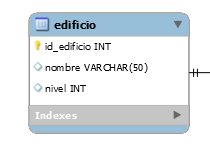
\includegraphics[width=.5\textwidth]{images/clases/Edificio.png}}
		\caption{Modelo de información del módulo Edificios.}
		\label{fig:edificio}
	\end{center}
\end{figure}

%--------------------------------------------------------------------------------
\begin{BusinessEntity}{edificio}{Edificio}
	
	\Battr{nombre}{Nombre}{\tdFrase}{Es el nombre con el que se registra el edificio}{\requerido}{\longitudMax{50}{caracteres}}{Caracteres admitidos: [A-Z] $|$ [a-z] $|$ [1-9] $|$ [á,é,é,ó,ú]  $|$ [Á,É,Í,Ó,Ú] $|$ \_ $|$ $-$ $|$ \textvisiblespace.}
	
	\Battr{nivel}{Nivel}{\tdNumerico}{Es el número de niveles totales que tiene el edificio}{\requerido}{\longitudMinMax{1}{caracteres}{2}{caracteres}}{Caracteres admitidos: [0-9].}
	
\end{BusinessEntity}
%--------------------------------------------------------------------------------

\subsection{Módulo Espacios: Descripción general}
En la figura~\ref{fig:espacios} se muestra la estructura de información que manejará el módulo Espacios.

\begin{figure}[htbp!]
	\begin{center}
		\fbox{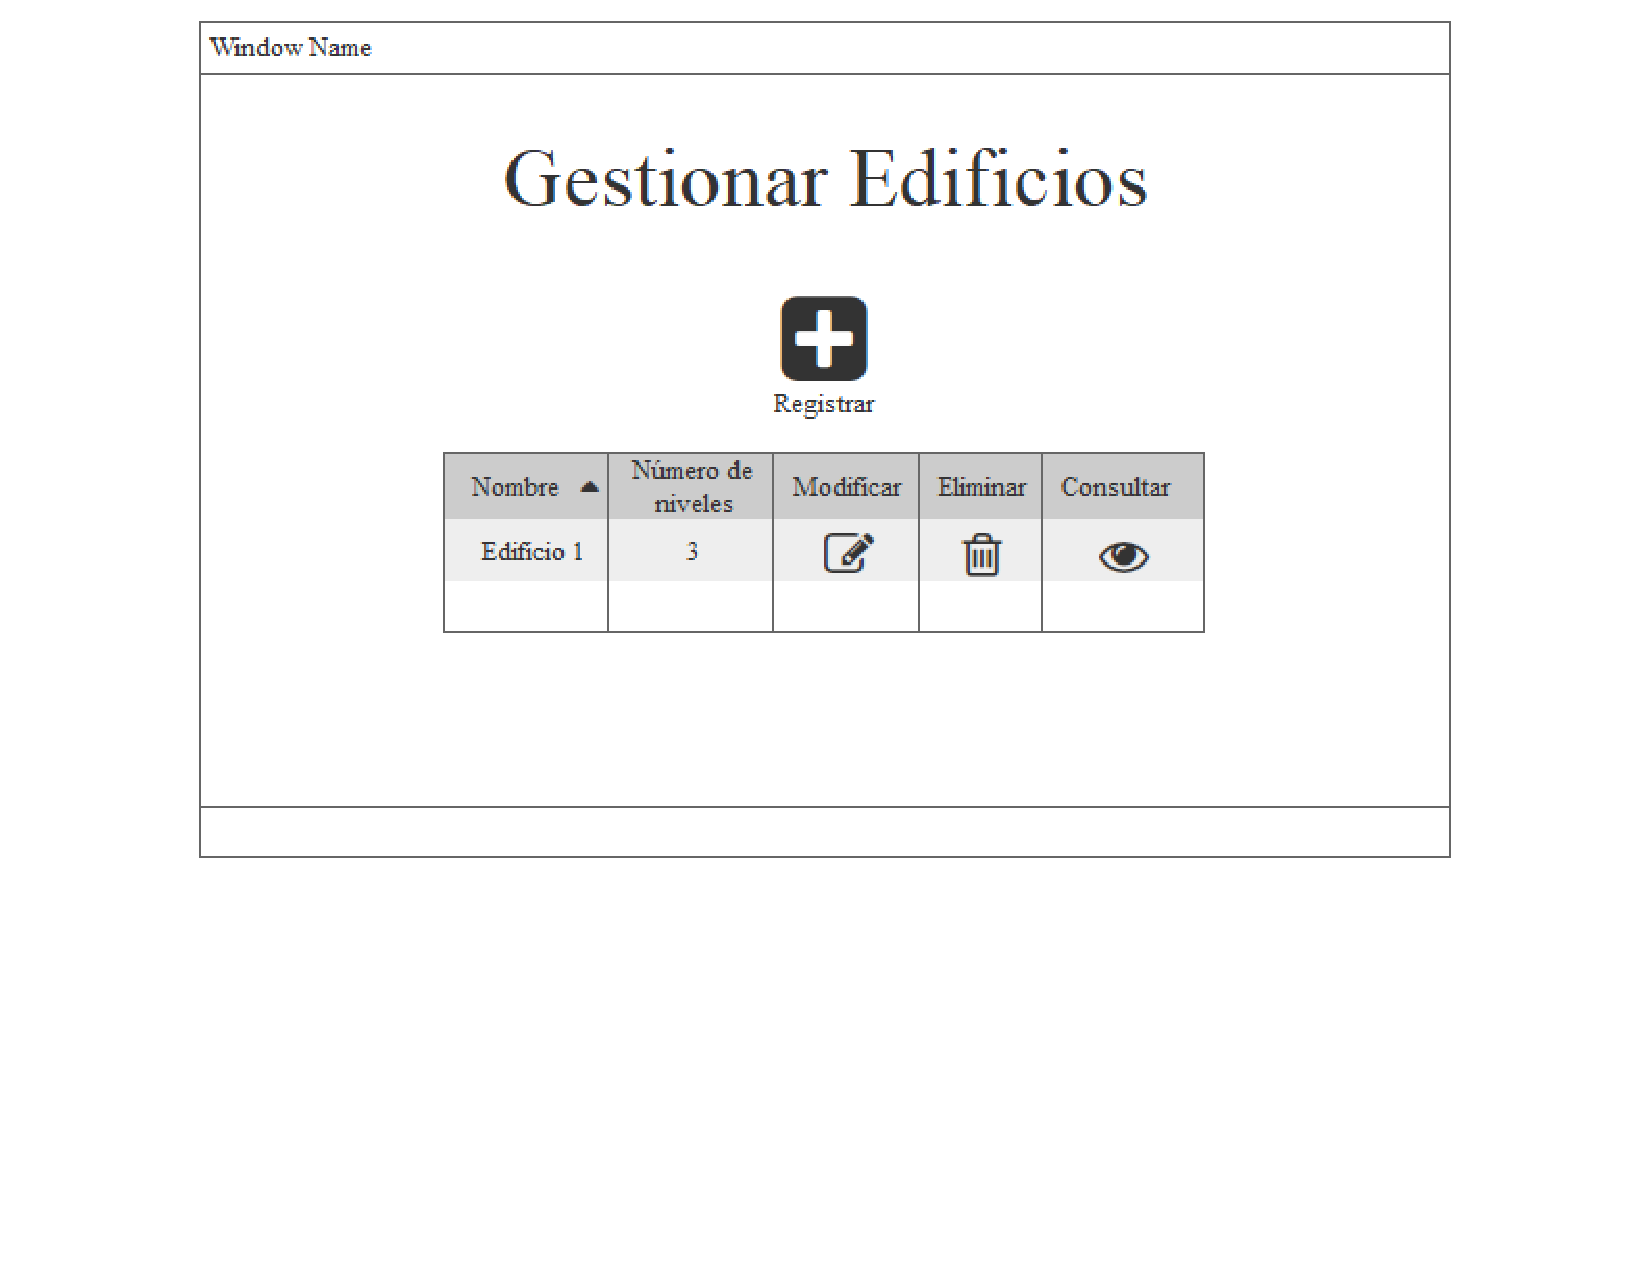
\includegraphics[width=.5\textwidth]{images/clases/Espacios.png}}
		\caption{Modelo de información del módulo de Espacios.}
		\label{fig:espacios}
	\end{center}
\end{figure}

%--------------------------------------------------------------------------------
\begin{BusinessEntity}{espacio}{Espacio}
	
	\Battr{nivel}{Nivel}{\tdNumerico}{Es el número que indica a que nivel del edificio corresponde el espacio}{\requerido}{\longitudMinMax{1}{caracteres}{2}{caracteres}}{Caracteres admitidos: [0-9].}
	
	\Battr{clave}{Clave}{\tdNumerico}{Es un número generado por la concatenación del número del edificio + número de nivel + el número del espacio}{calculado por el sistema}{Este atributo es de 4 caracteres exactamente. }{Caracteres admitidos: [0-9].}

	\Battr{numero}{Número}{\tdNumerico}{Es el número que se le asigna al espacio}{\requerido}{\longitudMinMax{1}{caracteres}{2}{caracteres}}{Caracteres admitidos: [0-9].}
	
	\Battr{nombre}{Nombre}{\tdFrase}{Es el nombre con el que se registra el espacio}{\requerido}{\longitudMax{50}{caracteres}}{Caracteres admitidos: [A-Z] $|$ [a-z] $|$ [1-9] $|$ \_ $|$ $-$ $|$ [á,é,é,ó,ú]  $|$ [Á,É,Í,Ó,Ú] $|$ \textvisiblespace.}
	
	\Battr{capacidad}{Capacidad}{\tdNumerico}{Es el número que define la capacidad de alumnos que permite el espacio}{\requerido}{\longitudMinMax{1}{caracteres}{2}{caracteres}}{Caracteres admitidos: [0-9].}
	
	\Battr{accesoDiscapacitados}{Acceso a discapacitados}{\tdBooleano}{Indica si el espacio es accesible para las personas con capacidades diferentes}{\requerido}
	
	\Battr{observaciones}{Observaciones}{\tdFrase}{Es una frase }{\requerido}{\longitudMax{150}{caracteres}}{Caracteres admitidos: [A-Z] $|$ [a-z] $|$ [1-9] $|$ \_ $|$ $-$ $|$ [á,é,é,ó,ú]  $|$ [Á,É,Í,Ó,Ú] $|$ \textvisiblespace.}
	
	\Battr{funciona}{En función}{\tdBooleano}{Indica si el espacio puede ser contemplado en la asignación de espacios para los grupos ofertados.}{\requerido}
	
\end{BusinessEntity}

%--------------------------------------------------------------------------------
\begin{BusinessEntity}{tipoLaboratorio}{Tipo de laboratorio}
	
		\Battr{nombreTipoLab}{Tipo de laboratorio}{\tdCatalogo}{Es el tipo de laboratorio que es un espacio catalogado como laboratorio, como son: \begin{itemize}
			\item Computación 
			\item Electrónica 
			\item Física 
			\item Programación 
			\item Redes 
			\item Sistemas
		\end{itemize}
	}{\requerido}
	
\end{BusinessEntity}

%--------------------------------------------------------------------------------
\begin{BusinessEntity}{tipoEspacio}{Tipo de espacio}
	
	\Battr{nombre}{Tipo de espacio}{\tdCatalogo}{Es el tipo de espacio que se registra, como son: \begin{itemize}
			\item Aula 
			\item Laboratorio 
		\end{itemize}
	}{\requerido}
	
\end{BusinessEntity}


%--------------------------------------------------------------------------------